\normaltrue \difficilefalse \tdifficilefalse
\correctionfalse

%\UPSTIidClasse{11} % 11 sup, 12 spé
%\newcommand{\UPSTIidClasse}{12}

\exer{Système bielle manivelle  $\star$ \label{CIN:01:B2:13:PTSI:12}}
\setcounter{question}{0}\marginnote{\xpComp{CIN}{01}}%\UPSTIcompetence[2]{B2-13}
\index{Compétence B2-13-PTSI}
\index{Bielle Manivelle}
\index{Moteur}
\ifcorrection
\else
\marginnote{\textbf{Pas de corrigé pour cet exercice.}}
\fi

\ifprof
\else
Soit le mécanisme suivant. 

\begin{marginfigure}
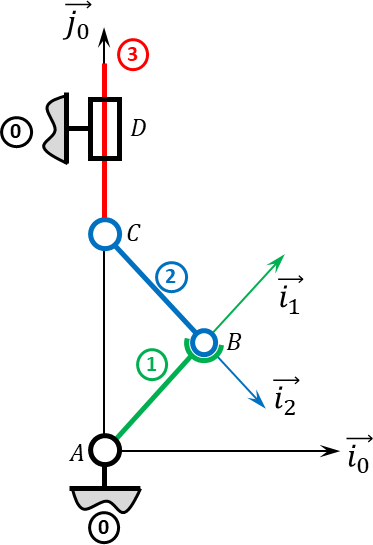
\includegraphics[width=0.6\linewidth]{12_01}
\end{marginfigure}
\fi


\question{Réaliser le paramétrage du mécanisme.}
\ifprof

\else
\fi


\ifprof
\else
\marginnote{Corrigé voir \ref{CIN:01:B2:13:PTSI:12}.}

\fi